\documentclass[]{article}
\usepackage[german]{babel}
\usepackage{graphicx}
\usepackage{tabularx}
\usepackage[backend=bibtex, natbib=true]{biblatex}
\usepackage{listings}
\usepackage{tikz}

\lstset{%
	basicstyle=\ttfamily\scriptsize,        % Code font, Examples: \footnotesize, \ttfamily
	keywordstyle=\color{blue!80!black},     % Keywords font ('*' = uppercase)
	commentstyle=\color{gray},              % Comments font
	numbers=left,                           % Line nums position
	numberstyle=\tiny,                      % Line-numbers fonts
	stepnumber=1,                           % Step between two line-numbers
	numbersep=5pt,                          % How far are line-numbers from code
	backgroundcolor=\color{gray!10!white},  % Choose background color
	frame=none,                             % A frame around the code
	tabsize=2,                              % Default tab size
	captionpos=b,                           % Caption-position = bottom
	breaklines=true,                        % Automatic line breaking?
	breakatwhitespace=false,                % Automatic breaks only at whitespace?
	showspaces=false,                       % Dont make spaces visible
	showstringspaces=false                  %
	showtabs=false,                         % Dont make tabls visible
	columns=flexible,                       % Column format
	morekeywords={},                        % Specific keywords
	stringstyle=\color{green!50!black},%
}%

\bibliography{bibliography}
%opening
%Here you can enter your names and titleof your report
\title{Weekly Reports}
\author{Luftqualität in Innenräumen - Gruppe 1}

\begin{document}

\maketitle

\begin{table}[h!]
	\centering
	\begin{tabular}{|c|c|c|}
		\hline
		{\textbf{Name}}				&		{\textbf{Matrikel Nr.}} & {\textbf{Arbeitsaufwand (h)}} \\
		\hline
		Friedrich Just				&		1326699 				&		\\
		\hline
		Stipe Knez				&		1269206 				&		\\
		\hline
		Lucas Merkert				&		1326709					&	20,00	\\
		\hline
		Achim Glaesmann				&		1309221					&		\\
		\hline
		Max-Rene Konieczka			&		1211092					&		\\
		\hline
		Can Cihan Nazlier			&		1179244					&		\\
		\hline
	\end{tabular}
	\caption{Arbeitsaufwand dieser Woche}
	\label{tab:worakload}
\end{table}



\section{Überblick}


\subsection{Friedrich Just}

\subsection{Stipe Knez}

\subsection{Lucas Merkert}
Über die Weihnachtsferien: Einarbeitung in die Funktionalität des Sensors CCS811:
\begin{itemize}
	\item Schreiben auf den Sensor über die Adresse 0x5A
	\begin{enumerate}
		\item Schreiben des Befehls 0x40 in das Register 0x01
		\item Bisher return 0 von HALWriteI2CPacket()
	\end{enumerate}
	\item Lesen des Sensor über die Adresse 0X5B
		\begin{enumerate}
			\item Lesen von 4 Bytes zum Lesen der CO2 und TVOC werte im Register 0x02
			\item Bisher return 0 von HALReadI2CPacket()
		\end{enumerate}
	\end{itemize}

Der Wake-Pin ist zurzeit an GND angeschlossen. Allerdings scheint noch etwas nicht zu funktionieren, diesen soll in der nächsten Woche geklärt werden. 
\begin{figure}[h]
	\centering
	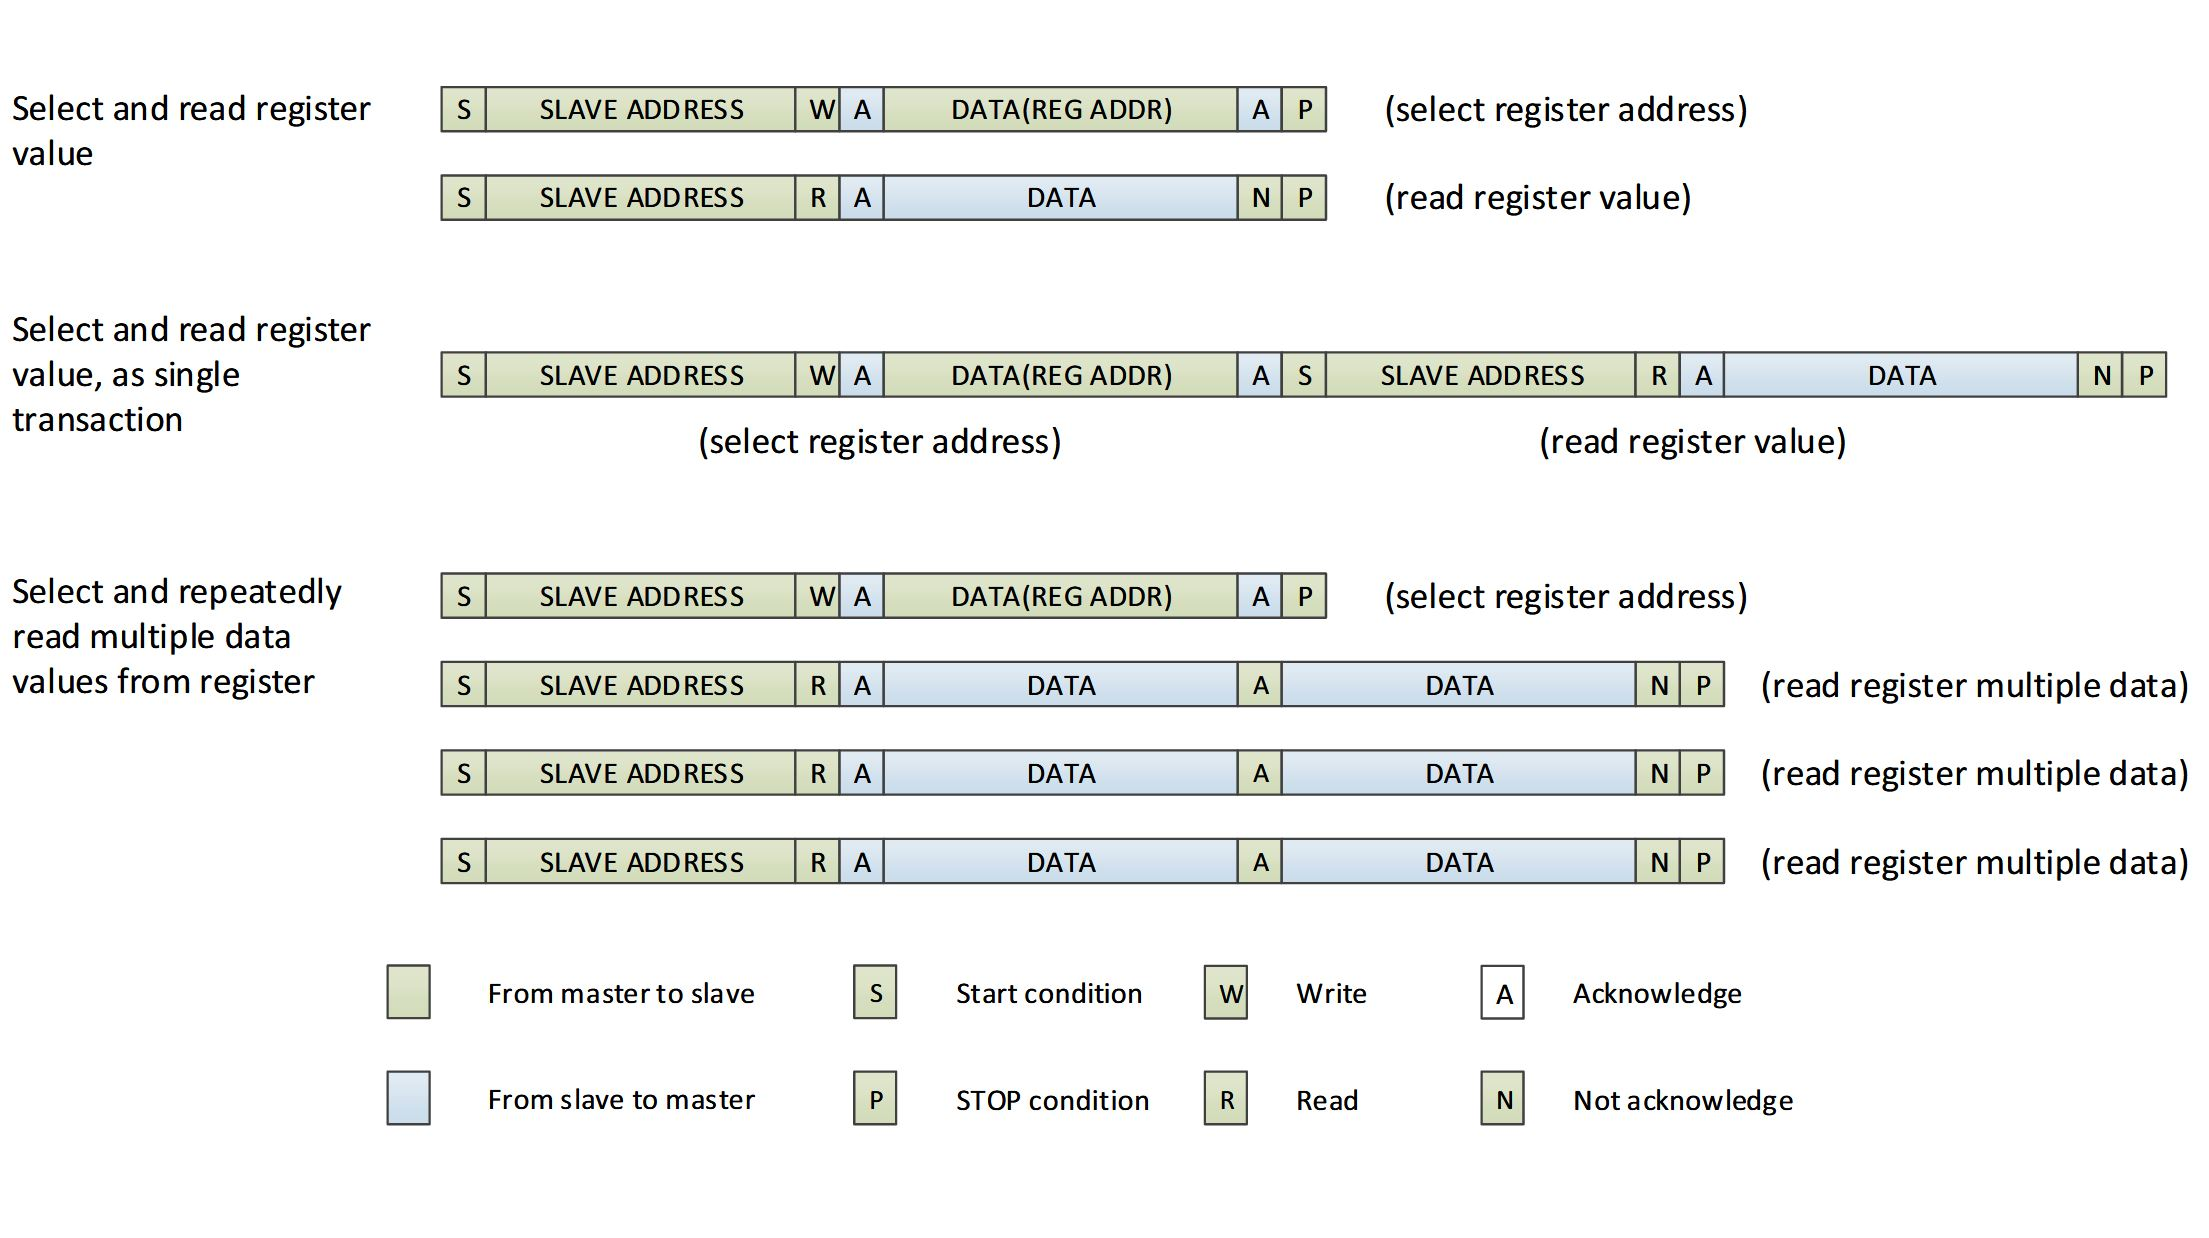
\includegraphics[scale=0.30]{images/i2c_ccs811}
	\caption{Funktionsweise der I2C-Packet Übertragung\cite{datasheetcss811}}
	\label{img:I2C_ccs811}
\end{figure}


\subsection{Achim Glaesmann}

\subsection{Max-Rene Konieczka}
Während zurzeit noch daran gearbeitet wird die Daten der Sensoren auszulesen, wurde zunächst versucht die zuvor mit Python erstellten Mockdaten, in unsere Datenbank einzulesen. Dafür haben wir das Serialport Package von Node sowie ein Programm zur Erstellung von virtuellen Ports verwendet. Es hat sich die Frage gestellt, ob und wie die Mockdaten in der Datenbank angezeigt werden könnten. Dies ist in Zusammenarbeit mit Stipe Knez passiert.
\subsection{Can Cihan Nazlier}

\printbibliography
%----------------------------------------------------------------------------
% Bibliography
%----------------------------------------------------------------------------	

\end{document}
